\chapter{Introduction}
\label{introchap}


In the mid-1960s, experimental physicist Raymond Davis Jr., in collaboration with theorist John Bahcall, placed a 100\,000 gallon tank of dry-cleaning fluid one mile underground in a mine in South Dakota. While this may seem like a peculiar thing to do, they had a very clear goal in mind: to determine the flux of electron neutrinos produced from nuclear fusion reactions in the Sun. When a high-energy electron neutrino passes by the nucleus of a chlorine atom (which are prevalent in the dry-cleaning fluid he used), there is a small chance that the chlorine atom will absorb the neutrino and convert into an argon ion. By counting the number of argon ions accumulated over time, Davis was able to determine the number of electron neutrinos captured in their tank, and compare to the theoretical expectation calculated by Bahcall's solar model. By 1968, the first results of the experiment were published: they were capturing about one-third fewer electron neutrinos than anticipated from the leading theory at the time \cite{Bahcall:1964gx,Davis:1968cp}. The experiment continued until 1994, repeatedly confirming the apparent discrepancy. In that time, theorists rushed to find a potential explanation, while experimentalists rushed to confirm the result with other experiments. On the theory side, it was determined that neutrinos of the electron flavor must oscillate into neutrinos of the muon and tau flavor as they pass through the Sun and the vacuum of space. On the experimental side, the result was confirmed by the Super-Kamiokande experiment in 1998 \cite{Super-Kamiokande:1998kpq} and the Sudbury Neutrino Observatory in 2001 \cite{Oser:2001rh}. The results are clear: although it is conserved in the Standard Model of particle physics, we know from these experiments that lepton flavor symmetry is violated in our universe. 

 While there is indirect evidence of physics beyond the Standard Model from astrophysical observations, no other direct-detection particle physics experiment has uncovered such a striking and persistent disagreement with the Standard Model paradigm. While the resolution -- flavor oscillations of neutrinos -- is straightforward, the source of this lepton flavor violation is still unknown. Many solutions have been proposed, such as heavy right-handed neutrinos and an additional Higgs boson with exotic properties \cite{Minkowski:1977sc,Magg:1980ut}. One of the difficulties with testing such theories is that neutrinos are electromagnetically neutral, which makes them particularly unwieldy in a lab environment. For every neutrino successfully captured in Davis' experiment, one billion trillion neutrinos passed straight through the tank unimpeded.

Luckily for experimentalists, electromagnetically {\it charged} leptons also exist: the electron ($e$), which is responsible for the inner-workings of all modern electronics; the muon ($\mu$), which decays in two millionths of a second but has nonetheless been used to image hard-to-reach locations such as volcanic caverns and hidden rooms within the pyramids; and the tauon ($\tau$), which decays in less than one trillionth of a second and, as far as we know, has no practical use (but is nonetheless of profound interest to the particle physics community!). Their charge makes these leptons much easier to study in experiments: the electromagnetic properties of the electron are the most precise measurements in all of physics, and those of the muon are not too far behind. But so far, according to both the Standard Model and modern experimental observations, the charged leptons do not appear to oscillate from one flavor to another. Nonetheless, it is possible to show that flavor violation in the neutrino sector leads directly to flavor violation in the charged lepton sector as well.

For a concrete example, consider the one-loop Feynman diagram depicting the decay of a muon to an electron and a photon $\mu \rightarrow e \gamma$ (Fig. \ref{fig:mu_e_gamma}). The corresponding branching fraction\footnote{For the uninitiated: {\it branching fraction} is the probability that a particle {\it branches}, or decays, to a specified final-state of other particles. ${\cal B}(\mu \rightarrow e\gamma)$ represents the {\it probability} that a muon decays to an electron and a photon.} for this process can be estimated as \cite{Bilenky:1977du}
\beq
    {\cal B}({\mu\rightarrow e\gamma}) \sim \frac{3}{32}\frac{\alpha}{\pi}\frac{(\Delta m_\nu^2)^2}{m_W^4}.
\eeq
The neutrino masses $m_{\nu_i}$ have never been measured directly and are predicted to be zero by the Standard Model. However, neutrino oscillation requires that they have non-zero mass, and observations of solar neutrinos predict a difference in the squares of the $e$ and $\mu$ neutrino masses of $| m_{\nu_\mu}^2-m_{\nu_e}^2| \approx (10~{\rm meV})^2$ \cite{ParticleDataGroup:2024cfk}. This corresponds to a branching fraction of ${\cal B}(\mu \rightarrow e\gamma) \approx 10^{-54}$. Meanwhile, the leading experimental bounds on the $\mu \rightarrow e\gamma$ decay come from the Mu to E Gamma (MEG) experiment, with a current limit on the branching fraction of ${\cal B}(\mu \rightarrow e\gamma) < 4.2\times 10^{-13}$. Evidently, there is a large gap to fill. The upgrade to MEG, MEG II, is anticipated to improve these bounds by ten-fold by the time of its completion in 2026. If the MEG experiment continues to be upgraded with a factor-of-ten increase in sensitivity each decade, we can expect an announcement of the discovery of the $\mu\rightarrow e\gamma$ decay mode via neutrino oscillations from the MEG XLI experiment some time in the 2400s. Let's not hold our breath.
\begin{figure}
    \centering
    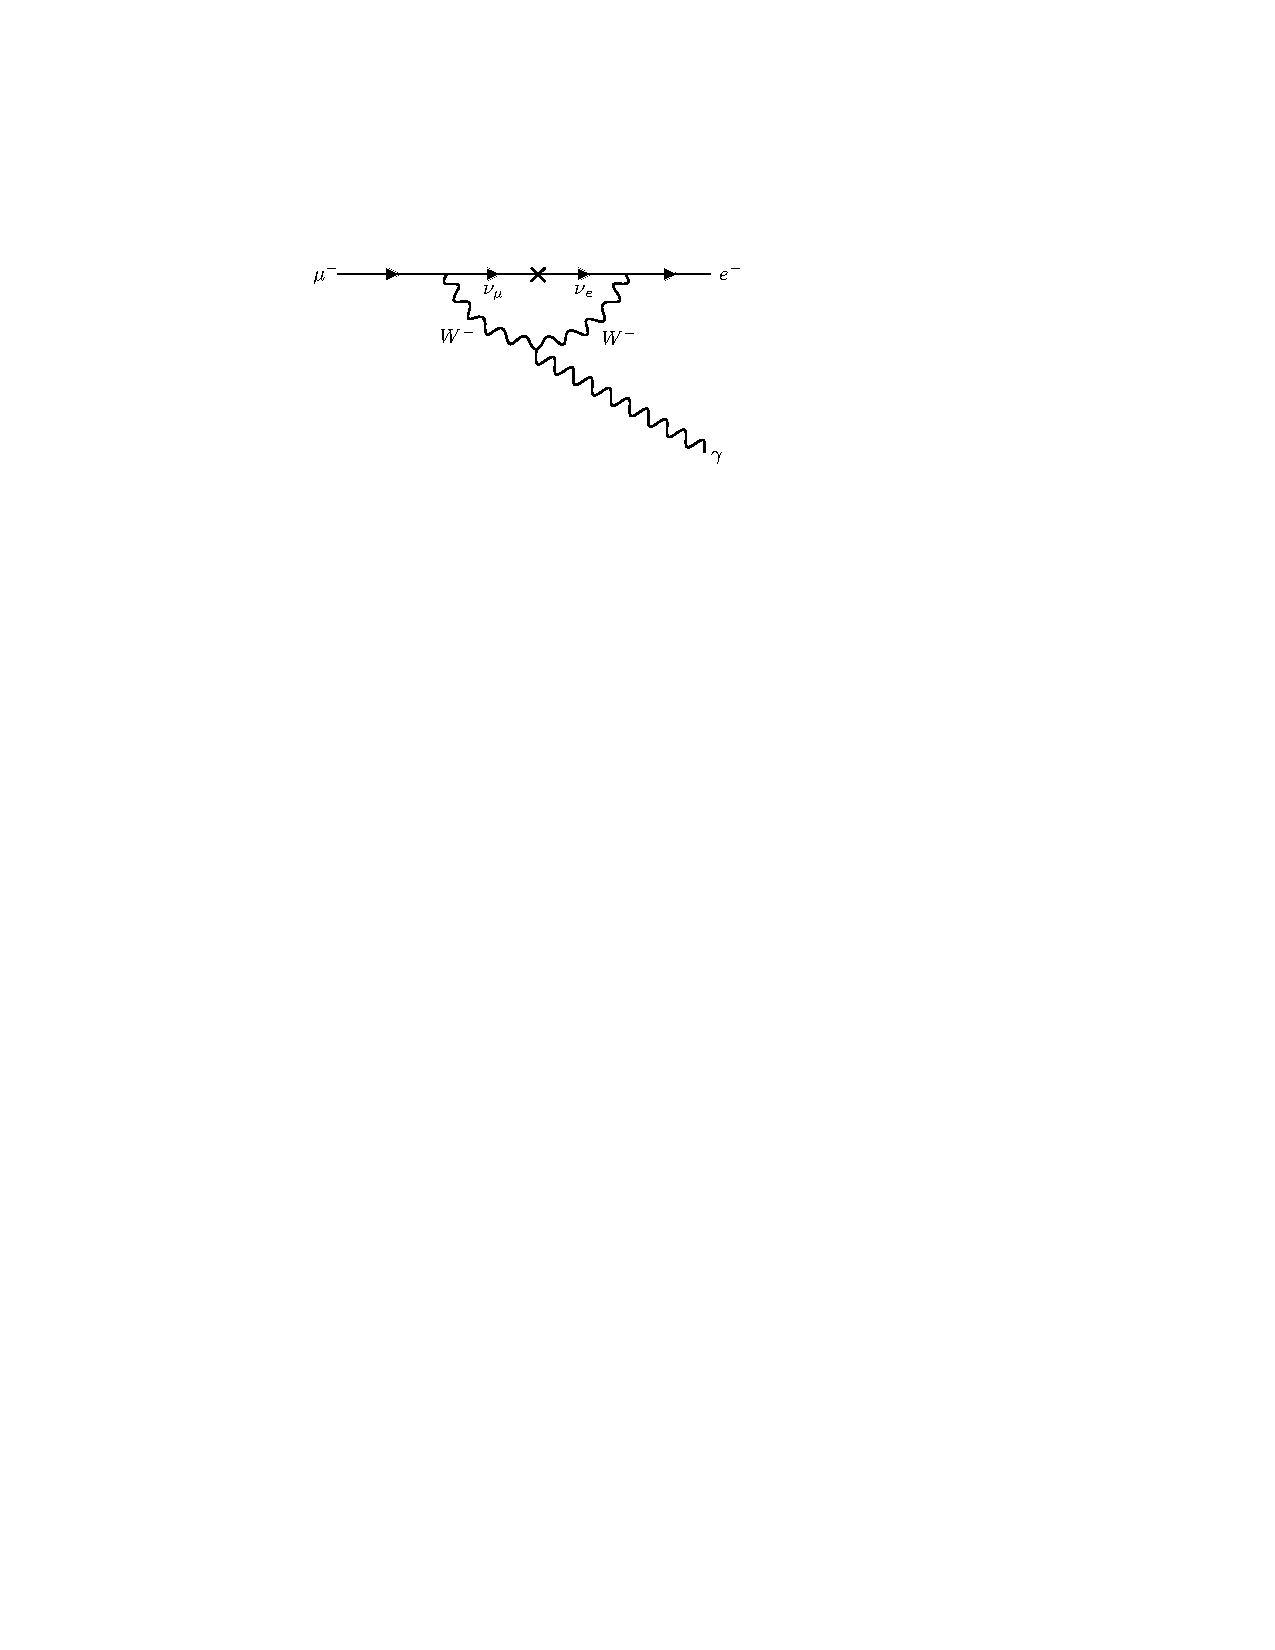
\includegraphics[width=0.6\linewidth]{figures/chapter1/mu_e_gamma.pdf}
    \caption{A Feynman diagram representing the LFV $\mu \rightarrow e\gamma$ decay mediated via neutrino oscillation.}
    \label{fig:mu_e_gamma}
\end{figure}

The honest hope of particle physicists is that we will detect evidence of the $\mu\rightarrow e\gamma$ decay mode long before then. If this occurs, it will evidently not be due to neutrino oscillations, but to some as-yet unknown process which exists beyond the Standard Model (and which may be responsible for the observed neutrino oscillations). Indeed, as we will explore in Chapter 2, it turns out to be very difficult to add new physics to the Standard Model {\it without} introducing charged lepton flavor violation (CLFV). 

The ubiquity of CLFV in extensions of the Standard Model makes it a promising avenue to search for new physics. After all, the charged leptons (and especially the electron) are much easier to detect and control than their neutral counterparts. But by the same token, if a CLFV signal {\it is} detected, the source of the flavor violation will likely remain unclear until more dedicated experiments are carried out. We have already seen this in the neutrino sector: there is a whole host of potential explanations for the existence and size of the neutrino masses, most of which can explain our observations while evading detection in other existing experiments. 

In this dissertation, we will explore constraints on the existence of particles with CLFV couplings. In Chapter \ref{fv_qft}, we will review some models which exhibit this behavior, namely models with LFV scalars and axion like particles (ALPs). In Chapter \ref{lfv}, we will examine the constraints one can place on these models in the context of LFV charged lepton decays, such as the $\mu \rightarrow e\gamma$ decay mode described in the Introduction. In Chapter 4, we will explore one possible production mechanism for such particles: coherent interactions between an electron or muon beam and a heavy nucleus. In Chapter \ref{alp_collider}, we will apply the results of Chapter \ref{upc} to place projected limits on the flavor-violating couplings of ALPs at various experiments involving lepton-nucleus collisions, and we will compare these to limits one can place from Higgs decays at the LHC. Finally, in Chapter \ref{bosons}, we will study production of dark $U(1)$ gauge bosons at lepton-nucleus collision experiments, and resulting limits one can obtain on the gauge coupling. The code to generate the figures in this thesis can be found in the GitHub repository \href{https://github.com/rmarcarelli/thesis/}{github.com/rmarcarelli/thesis/} \cite{MarcarelliGithub2025}.
